\documentclass[hidelinks,12pt]{article}
\usepackage[left=0.25cm,top=1cm,right=0.25cm,bottom=1cm]{geometry}
%\usepackage[landscape]{geometry}
\textwidth = 20cm
\hoffset = -1cm
\usepackage[utf8]{inputenc}
\usepackage[spanish,es-tabla]{babel}
\usepackage[autostyle,spanish=mexican]{csquotes}
\usepackage[tbtags]{amsmath}
\usepackage{nccmath}
\usepackage{amsthm}
\usepackage{amssymb}
\usepackage{mathrsfs}
\usepackage{graphicx}
\usepackage{subfig}
\usepackage{standalone}
\usepackage[outdir=./Imagenes/]{epstopdf}
\usepackage{siunitx}
\usepackage{physics}
\usepackage{color}
\usepackage{float}
\usepackage{hyperref}
\usepackage{multicol}
%\usepackage{milista}
\usepackage{anyfontsize}
\usepackage{anysize}
%\usepackage{enumerate}
\usepackage[shortlabels]{enumitem}
\usepackage{capt-of}
\usepackage{bm}
\usepackage{relsize}
\usepackage{placeins}
\usepackage{empheq}
\usepackage{cancel}
\usepackage{wrapfig}
\usepackage[flushleft]{threeparttable}
\usepackage{makecell}
\usepackage{fancyhdr}
\usepackage{tikz}
\usepackage{bigints}
\usepackage{scalerel}
\usepackage{pgfplots}
\usepackage{pdflscape}
\pgfplotsset{compat=1.16}
\spanishdecimal{.}
\renewcommand{\baselinestretch}{1.5} 
\renewcommand\labelenumii{\theenumi.{\arabic{enumii}})}
\newcommand{\ptilde}[1]{\ensuremath{{#1}^{\prime}}}
\newcommand{\stilde}[1]{\ensuremath{{#1}^{\prime \prime}}}
\newcommand{\ttilde}[1]{\ensuremath{{#1}^{\prime \prime \prime}}}
\newcommand{\ntilde}[2]{\ensuremath{{#1}^{(#2)}}}

\newtheorem{defi}{{\it Definición}}[section]
\newtheorem{teo}{{\it Teorema}}[section]
\newtheorem{ejemplo}{{\it Ejemplo}}[section]
\newtheorem{propiedad}{{\it Propiedad}}[section]
\newtheorem{lema}{{\it Lema}}[section]
\newtheorem{cor}{Corolario}
\newtheorem{ejer}{Ejercicio}[section]

\newlist{milista}{enumerate}{2}
\setlist[milista,1]{label=\arabic*)}
\setlist[milista,2]{label=\arabic{milistai}.\arabic*)}
\newlength{\depthofsumsign}
\setlength{\depthofsumsign}{\depthof{$\sum$}}
\newcommand{\nsum}[1][1.4]{% only for \displaystyle
    \mathop{%
        \raisebox
            {-#1\depthofsumsign+1\depthofsumsign}
            {\scalebox
                {#1}
                {$\displaystyle\sum$}%
            }
    }
}
\def\scaleint#1{\vcenter{\hbox{\scaleto[3ex]{\displaystyle\int}{#1}}}}
\def\bs{\mkern-12mu}


\title{Segunda solución linealmente independiente \\ \large {Tema 2 - Matemáticas Avanzadas de la Física}\vspace{-3ex}}

\author{M. en C. Gustavo Contreras Mayén}
\date{ }

\pagestyle{fancy}
\fancyhf{}
\rhead{Curso MAF}
\lhead{\leftmark}
\rfoot{\thepage}
\setlength{\headheight}{16pt}%


\begin{document}
\maketitle
\fontsize{14}{14}\selectfont

\section{Independencia lineal}

\subsection{Ejercicio 1}

\begin{ejemplo}
Si las funciones $y_{1}$ y $y_{2}$ son soluciones linealmente independientes de:
\begin{align*}
\sderivada{y} + p(x) \, \pderivada{y} + q(x) \, y = 0
\end{align*}
Demuestra que $c_{1} \, y_{1}$ y $c_{2} \, y_{2}$ también son soluciones linealmente independientes, siempre que $c_{1} \neq 0$ y $c_{2} \neq 0$.
\par
Revisemos el Wronskiano:
\begin{align*}
W = \mdet{
c_{1} \, y_{1} & c_{2} \, y_{2} \\ 
c_{1} \, \pderivada{y}_{1} & c_{2} \, \pderivada{y}_{2}
}
\end{align*}
Desarrollemos el determinante:
\begin{align*}
W &= \big[ c_{1} \, y_{1} * c_{2} \, \pderivada{y}_{2} \big] - \big[ c_{1} \, \pderivada{y}_{1} * c_{2} \, y_{2} \big] = \\[0.5em] 
&= c_{1} \, c_{2} \, y_{1} \, \pderivada{y}_{2} - c_{1} \, c_{2} \pderivada{y}_{1} \, y_{2} = \\[0.5em] 
&= c_{1} \, c_{2} \, \big[ y_{1} \, \pderivada{y}_{2} - \pderivada{y}_{1} \, y_{2} \big] \\[0.5em] 
&= c_{1} \, c_{2} \, W(y_{1}, y_{2})
\end{align*}

Dado que $y_{1}$ y $y_{2}$ son linealmente independientes, entonces $W(y_{1}, y_{2}) \neq 0$, además de que $c_{1} \neq 0$ y $c_{2} \neq 0$, se tiene que:
\begin{align*}
W(c_{1} \, y_{1}, c_{2} \, y_{2}) = c_{1} \, c_{2} \, W(y_{1}, y_{2}) \neq 0
\end{align*}
por tanto $c_{1} \, y_{1}$ y $c_{2} \, y_{2}$ son linealmente independientes.
\end{ejemplo}

\subsection{Ejercicio 2}

\begin{ejemplo}
Las funciones $\sin x$, $e^{x}$ y $e^{-x}$ son linealmente independientes, ya que ninguna de ellas puede escribirse como una combinación lineal de las otras dos. Demuestra que el Wronskiano de las tres funciones se anula pero en puntos aislados.
\par
Tenemos que desarrollar el Wronskiano de las tres funciones, y revisar en qué tipo de puntos aislados se anula el determinante.
\begin{align*}
W = \mdet{
\sin x & e^{x} & e^{-x} \\
\cos x & e^{x} & -e^{-x} \\
-\sin x & e^{x} & e^{-x}
}
\end{align*}

Calculamos el determinante como aprendimos en álgebra lineal:
\begin{align*}
W &= \sin x \, \mdet{
e^{x} & -e^{x} \\
e^{x} & e^{x} \\
} - e^{x} \mdet{
\cos x & -e^{-x} \\
-\sin x & e^{-x}
} + \\[0.5em]
&+e^{-x} \mdet{
\cos x & e^{x} \\
-\sin x & e^{x}
}
\end{align*}

El Wronskiano es:
\begin{align*}
W &= 2 \, \sin x - e^{x} \bigg[ e^{-x} \, \cos x - e^{x} \, \sin x \bigg] \\[0.5em]
&+ e^{-x} \bigg[ e^{x} \, \cos x + e^{-x} \, \sin x \bigg] = \\[0.5em] 
&= 2 \, \sin x - (\cos x -\sin x) + (\cos x + \sin x) = \\[0.5em] 
&= 4 \, \sin x
\end{align*}

Revisamos en qué puntos el Wronskiano se anula, al tener la función $\sin x$, sabemos que se anula en los puntos que son múltiplos enteros de $\pi$, por tanto el Wronskiano se anula en:
\begin{align*}
W = 0 \hspace{1.5cm} x = \pm n \, \pi, \hspace{0.5cm} n = 0, 1, 2, \ldots
\end{align*}
\end{ejemplo}

\section{Segunda solución independiente}

\subsection{Ejercicio 3 - Con integrales}

\begin{ejemplo}
Una solución de la ecuación diferencial de Laguerre:
\begin{align*}
x \, \sderivada{y} + (1 - x) \, \pderivada{y} + n \, y = 0
\end{align*}
para $n = 0$ es $y_{1}(x) = 1$. Utilizando la ecuación:
\begin{align*}
y_{2}(x) =  y_{1} \: (x) \int^{x} \dfrac{\exp \left[ \displaystyle - \int^{x_{2}} P(x_{1}) \: \dd{x_{1}} \right]}{[y_{1}(x_{2})]^{2}} \dd{x_{2}}
\end{align*}
desarrolla una segunda solución linealmente independiente. Exhibe explícitamente el término logarítmico de la solución.
\par
Ajustamos la ED inicial para dejarla en el formato:
\begin{align*}
\sderivada{y} + p(x) \, \pderivada{y} + q(x) \, y = 0
\end{align*}

por tanto:
\begin{align*}
\sderivada{y} + \dfrac{(1 - x)}{x} \, \pderivada{y} + \dfrac{n}{x} \, y = 0
\end{align*}

Por lo que en este caso:
\begin{align*}
p(x) = \dfrac{(1 - x)}{x} = \dfrac{1}{x} - 1
\end{align*}
que sustituiremos junto con $y_{1}(x)$ en la expresión que nos dará la segunda solución $y_{2}(x)$:
\begin{align*}
y_{2}(x) =  (1) \, \int^{x} \dfrac{\exp \left[ \displaystyle - \int^{x_{2}} \left( \dfrac{1}{x} - 1 \right) \: \dd{x_{1}} \right]}{[(1)]^{2}} \dd{x_{2}}
\end{align*}

Resolvemos primero la integral del argumento exponencial. La integral del argumento exponencial es:
\begin{align*}
- \int^{x} p(\pderivada{x}) \dd{\pderivada{x}} =  - \int^{x} \bigg[ \dfrac{1}{\pderivada{x}} - 1 \bigg] \dd{\pderivada{x}}=  - \ln x + x
\end{align*}

Que ahora sustituimos en la segunda integral para la solución, así tendremos que:
\begin{align*}
y_{2} (x) = \int \exp(- \ln x + x ) \dd{x} =  \int \dfrac{1}{x} \, e^{x} \dd{x}
\end{align*}

Vemos que en el integrando tenemos $1/x$, que de acuerdo a lo visto en Cálculo II, la antiderivada es $\ln x$, que es el factor logarítmico que nos piden mostrar explícitamente, pero hay que hacer un ajuste en el integrando para mantener ese factor logarítmico.
\par
La función exponencial la podemos expresar en términos de una serie de potencias:
\begin{align*}
e^{x} = \sum_{k=0}^{\infty} =  1 + x + \dfrac{x^{2}}{2!} + \dfrac{x^{3}}{3!} + \dfrac{x^{4}}{4!} + \ldots
\end{align*}

Entonces usamos esta expresión en el integrando:
\begin{align*}
\int \dfrac{1}{x} \, e^{x} \dd{x} = \int \dfrac{1}{x} \, \bigg[ 1 + x + \dfrac{x^{2}}{2!} + \dfrac{x^{3}}{3!} + \ldots \bigg] \dd{x}
\end{align*}

Multiplicamos los términos:
\begin{align*}
y_{2} = \int \bigg[ \dfrac{1}{x} + 1 + \dfrac{x}{2!} + \dfrac{x^{2}}{3!} + \ldots \bigg] \dd{x}
\end{align*}

Calculamos la integral de cada sumando:
\begin{align*}
y_{2} =  \ln (x) + x + \dfrac{x^{2}}{2 \cdot 2!} + \dfrac{x^{3}}{3 \cdot 3!} + \ldots
\end{align*}

Simplificando los términos:
\begin{align*}
y_{2} =  \ln (x) + \sum_{n=1}^{\infty} \dfrac{x^{n}}{n \cdot n!}
\end{align*}

En donde se muestra explícitamente el término logarítmico de la segunda solución linealmente independiente.
\end{ejemplo}

\subsection{Ejercicio 4 - Con series}

\begin{ejemplo}

Encuentra los primeros términos del desarrollo en series de potencias en torno al punto regular singular $x = 0$ de la solución general de
\begin{align*}
x^{2} \sderivada{y}  - x \, \pderivada{y} + (1 - x) \, y = 0, \hspace{1cm} x > 0
\end{align*} 

Se puede demostrar (trabajo moral) que ocupando el método de Frobenius la ecuación de índices es:
\begin{align*}
r^{2} - 2 \, r + 1 = 0
\end{align*}
donde las raíces son: $r_{1} = r_{2} = 1$. Con $r_{1} = 1$ se obtiene (trabajo moral) una solución en términos de una serie de potencias:
\begin{align*}
y_{1}(x) &= x + x^{2} + \dfrac{x^{3}}{4} + \dfrac{x^{4}}{36} + \dfrac{x^{5}}{576} + \ldots \\[1em]
&= \sum_{k=0}^{\infty} \dfrac{1}{(k!)^{2}} \, x^{k+1}
\end{align*}

Ya mencionamos que para obtener una segunda solución linealmente independiente $y_{2}(x)$, con $x_{0}=0$ la segunda solución es de la forma:
\begin{align*}
y_{2} (x) = y_{1}(x) \, \ln (x) + \sum_{n=1}^{\infty} b_{n} \, x^{n+1}
\end{align*}

Lo que debemos de hacer es determinar los coeficientes $b_{n}$, sustituyendo $y_{2}(x)$ directamente en la ED inicial. Por lo que tendremos que diferenciar $y_{2}$ hasta en dos ocasiones, para luego sustituir en la ED.
\begin{align*}
\pderivada{y}_{2} &= \pderivada{y}_{1} \, \ln x + x^{-1} \, y_{1} + \sum_{n=1}^{\infty} (n + 1) \, b_{n} \, x^{n} \\[1em]
\sderivada{y}_{2} &= \sderivada{y}_{1} \, \ln x + x^{-2} \, y_{1} + 2 \, x^{-1} \, \pderivada{y} + \sum_{n=1}^{\infty} n (n + 1) \, b_{n} \, x^{n-1}
\end{align*}

Que sustituimos en la ED inicial:
\begin{align*}
&x^{2} \left[ \sderivada{y}_{1} \, \ln x + x^{-2} \, y_{1} + 2 \, x^{-1} \, \pderivada{y}_{1} + \sum_{n=1}^{\infty} n (n + 1) \, b_{n} \, x^{n-1} \right] + \\[1em]
&- x \left[ \pderivada{y}_{1} \, \ln x + x^{-1} \, y_{1} + \sum_{n=1}^{\infty} (n + 1) \, b_{n} \, x^{n} \right] + \\[0.5em]
&+ (1 - x) \left[ y_{1} \, \ln x + \sum_{n=1}^{\infty} b_{n} \, x^{n+1} \right] = 0
\end{align*}
Factorizamos términos:
\fontsize{12}{12}\selectfont
\begin{align*}
&x^{2} \left[ \sderivada{y}_{1} \, \ln x + x^{-2} \, y_{1} + 2 \, x^{-1} \, \pderivada{y} + \sum_{n=1}^{\infty} n (n + 1) \, b_{n} \, x^{n-1} \right] + \\[1em]
&- x \left[ \pderivada{y}_{1} \, \ln x + x^{-1} \, y_{1} + \sum_{n=1}^{\infty} (n + 1) \, b_{n} \, x^{n+1} \right] + \\[0.5em]
&+ (1 - x) \left[ y_{1} \, \ln x + \sum_{n=1}^{\infty} b_{n} \, x^{n+1} \right] = 0
\end{align*}
% \begin{tikzpicture}[overlay]
% \draw [color=red] (0.9, 3.9) rectangle (3, 5.3);
% \draw [color=red] (1, 2) rectangle (3.3, 3.5);
% \draw [color=red] (1, 0.3) rectangle (4.3, 1.8);
% \end{tikzpicture}
Tenemos entonces:
\begin{align*}
\bigg[ x^{2} &\, \sderivada{y}_{1} - x \, \pderivada{y}_{1} + (1 - x) \, y_{1} \bigg] \, \ln x - 2 \, y_{1} +  2 \, x \, \pderivada{y}_{1} + \\[1em]
& + \sum_{n=1}^{\infty} n (n + 1) \, b_{n} \, x^{n+1} - \sum_{n=1}^{\infty} (n + 1) \, b_{n} \, x^{n+1} + \\[1em]
&+ \sum_{n=1}^{\infty} b_{n} \, x^{n+1} - \sum_{n=1}^{\infty} b_{n} \, x^{n+2} = 0
\end{align*} 
Notemos que el factor frente a $\ln x$:
\begin{align*}
\bigg[ x^{2} &\, \sderivada{y}_{1} - x \, \pderivada{y}_{1} + (1 - x) \, y_{1} \bigg]
\end{align*}
es justamente el lado izquierdo de la ED inicial con $y = y_{1}$. Como $y_{1}$ es solución, este factor se anula.

\par
Con la observación anterior y haciendo un corrimiento de los índices de las sumas, podemos escribir la ecuación como:
\begin{align*}
2 \, x \, \pderivada{y}_{1} -  2 \, y_{1} + b_{1} \, x^{2} +  \sum_{k=2}^{\infty} \big( k^{2} \, b_{k} - b_{k-1} \big) \, x^{k+1} = 0
\end{align*}

Para identificar los coeficientes $b_{k}$ y $b_{k-1}$ de modo que podamos igualarlos a cero, debemos de sustituir $y_{1}$ en su desarrollo en serie de potencias, así como $\pderivada{y}_{1}$. Entonces:
\begin{align*}
y_{1}(x) &= \sum_{k=0}^{\infty} \dfrac{1}{(k!)^{2}} \, x^{k+1}\\[0.5em] 
\pderivada{y}_{1} (x) &= \sum_{k=0}^{\infty} \dfrac{(k+1) \, x^{k}}{(k!)^{2}}
\end{align*}

Sustituyendo las series en la ecuación que estamos desarrollando:
\begin{align*}
&\sum_{k=0}^{\infty} \dfrac{2(k + 1) - 2}{(k!)^{2}} \, x^{k+1} + b_{1} \, x^{2} + \\[0.5em]
&+ \sum_{k=2}^{\infty} \bigg[ k^{2} \, b_{k} - b_{k-1} \bigg] \, x^{k+1} = 0
\end{align*}

Separamos los términos $k = 0$ y $k = 1$, para luego agrupar los términos semejantes:
\begin{align*}
(2 + b_{1}) \, x^{2} + \sum_{k=2}^{\infty} \bigg[ \dfrac{2 \, k}{(k!)^2} + k^{2} \, b_{k} - b_{k-1} \bigg] \, x^{k+1} = 0
\end{align*}

Ahora igualamos a cero los coeficientes de esta expresión. Tenemos entonces que:
\begin{align*}
(2 + b_{1}) =& \, 0 \\[1em]
\dfrac{2 \, k}{(k!)^2} + k^{2} \, b_{k} - b_{k-1} =& \, 0
\end{align*}

Por lo que los términos son:
\begin{align*}
b_{1} &= -2 \\[0.5em]
b_{k} &= \dfrac{1}{k^{2}} \left[ b_{k-1} - \dfrac{2 \, k}{(k!)^{2}} \right]
\end{align*}

Por lo que ya podemos calcular los otros dos términos que nos pide el enunciado del ejercicio, es decir, $k = 2, 3$:
\begin{align*}
b_{2} &= \dfrac{1}{2^{2}} [b_{1} - 1] = - \dfrac{3}{4} \\[0.5em]
b_{3} &= \dfrac{1}{9} \left[ -\dfrac{3}{4} - \dfrac{6}{36} \right] = - \dfrac{11}{108}
\end{align*}

Por tanto, una segunda solución linealmente independiente de la ED inicial es:
\begin{align*}
y_{2}(x) = y_{1}(x) \, \ln x - 2 \, x^{2} - \dfrac{3 \, x^{3}}{4} - \dfrac{11 \, x^{4}}{108} + \ldots
\end{align*}

Al graficar las soluciones tenemos la siguiente figura:
\begin{figure}
   \centering
   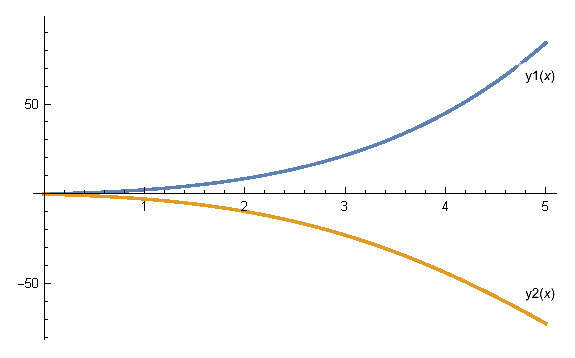
\includegraphics[scale=1]{Imagenes/Segunda_Solucion_Series_01.eps}
   \caption{Sumas parciales que aproximan las soluciones al ejercicio.}
\end{figure}
\end{ejemplo}
\end{document}